\documentclass{article}
\usepackage[utf8]{inputenc}
\usepackage{apacite}
\usepackage{graphicx} 
\usepackage{pdflscape}
\usepackage{url}



\graphicspath{{figures/}}

\title{Expert-Novice Spatiotemporal Pointing in Augmented Reality Music Teaching Systems}
\author{Jordan Aiko Deja}

\begin{document}
%\maketitle
\begin{center}
\large \textbf{Spatiotemporal Pointing in Augmented Reality Music Teaching Systems}
\\            
\vspace{0.5cm}\\
A Research Proposal\\
\vspace{0.5cm}
\textbf{Jordan Aiko Deja}\\
jordan.deja@famnit.upr.si\\
\vspace{0.5cm}
\textbf{Matjaž Kljun\\
Klen Čopič Pucihar}\\
Advisors\\
\vspace{0.5cm}
\today
\vspace{0.5cm}
\end{center}

\begin{abstract}
     Spatiotemporal pointing allows the user to touch base with a moving target within a limited time frame especially in a virtual space. In this given short window, the user has limited time to move, control its movement and even process the type of corresponding response that they should render. This phenomenon can be observed in any environment augmented by visual or audio cues - environments that require timely precision, rhythm and synchronization. Similarly, error rates of these spatiotemporal elements are commonly observed but are not properly modelled in order to mitigate them. Movements and precision are recognized differently by the computer as there are other considerations beyond flat surfaces and Fitts' Law. Spatiotemporal Pointing aims to address this gap for immersive spaces in Virtual, Augmented and Mixed Reality. With AR-based Music Teaching Applications becoming more prevalent yet not entirely adopted by practitioners and beginners, there is an open clamour for more usable learning systems. This research attempts to understand spatiotemporal pointing analysis and modeling in augmented reality music teaching systems between Experts and Novices. Future work shall investigate and understand their learning habits and patterns.  These then can be used to identify, design and develop better interfaces that mitigate the curve in their music learning experiences. 
\end{abstract}

\section{Introduction}
Temporal pointing refers to having a target that is about to appear within a limited time window for the user to response \cite{lee2016website}. Spatial pointing on the other hand requires the user to have control of the movement in an immersive space. As such Spatiotemporal pointing combines these two principles and is referred to as the movement of a user in an immersive environment as a response to a stimulus that is driven by a limited amount of time for selection. In such environments, there are many considerations that need to be understood. To maintain the temporal element, an immersive space needs to have an internal time-keeping mechanism, a response-execution stage, input processing done automatically all placed in a virtual non 2-dimensional space. There is a lot of work being done in this area with the aim of investigating and understanding human cognitive load, improving the accuracy in the rendering and performance of visual elements and discovering novel implications that minimise latency.\\

Innovations in spatiotemporal pointing contributes to Computational HCI. Since immersive environments are computer-generated, it is indeed vital to automate and streamline the processes that improve the modelling of the activities that happen in these environments such as spatiotemporal pointing. Virtual, Augmented and Mixed Reality environments are examples of ideal case studies in investigating spatiotemporal pointing. There are various related work seen in the succeeding section which has done formative studies on modelling, predicting, simulating action and reaction in such spaces. These studies have provided contribute to allowing us to understand (1) how objects move and collide in virtual spaces, (2) how users respond to these objects and (3) how we can foster design affordances that improve their performance. \\

A lot of music teaching systems have been built with augmented and virtual reality as a medium for innovation. There are notable augmented reality piano teaching systems that have been tested and investigated on such as the work of \cite{rogers2014piano, sun2018mr, birhanu2017keynvision}. These works have used overlaid and augmented visualizations in training the users with time-specific key presses. Such works improve the design as seen from their findings. However, cognitive load, user response time have not been carefully modelled or observed in the usage of the participants in these studies. This research attempts to address these gaps on building spatiotemporal models in these augmented reality music teaching systems. 
\section{Related Work}
There are only related work on spatio and temporal pointing in augmented and virtual reality spaces. There seems to be barely any research work on AR music teaching systems as the space is relatively new and has significant potential.\\
\begin{itemize}
\item The study of \cite{lee2016modelling} attempts to model error rates in temporal pointing. The tasks and experiments are done involving an object in an immersive spatial space. User reactions and actions like intercepting a ball where observed. Their study contributed on discussing theoretical assumptions on having an internal clock, response execution, input processing and others. Their findings mentioned selected methods between physical and touchscreenn buttons in gaming performance such as touch-down, touch-maximum, touch-release, key-press, key-release. These experiments were done with temporal games like Flappy Bird. Difficulty in participants were observed and opens the possibilities to discussing and modelling their actions, reactions in these temporal environments.
\begin{figure}[t]
\centering
 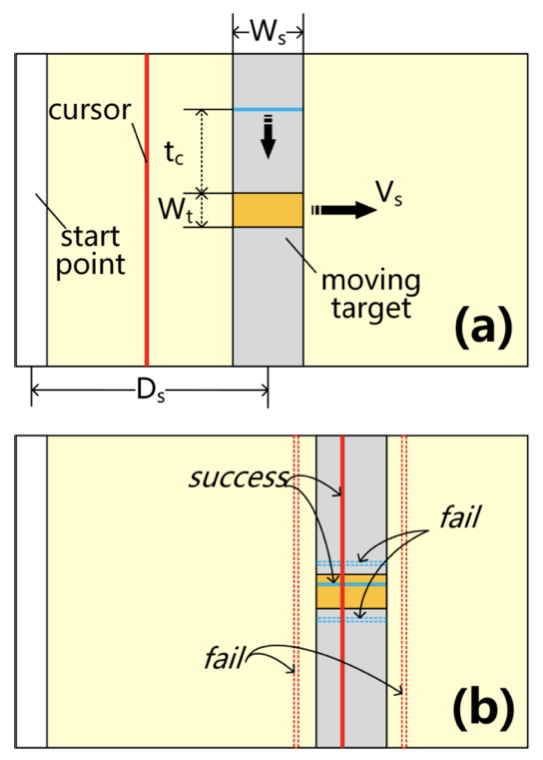
\includegraphics[width=4cm]{figures/spatiotemporalmovingtargetselection.png}
    \caption{Illustrating Spatiotemporal Task Selection with moving targets as seen in the work of \cite{lee2016modelling}.
 }\label{fig:spatiotemporaltask}
\end{figure}
\item The study of \cite{lee2017boxer}, investigated on multimodal collision of virtual objects. They compared temporal pointing vs virtual batting in terms of spatial precision in collisions. This was on a virtual ball game and not on a music teaching system.

\begin{figure}[t]
\centering
 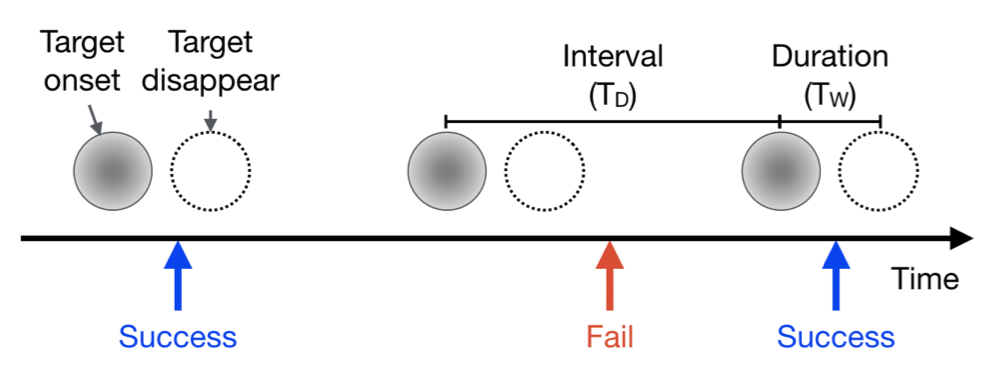
\includegraphics[width=8cm]{figures/boxmodel.png}
    \caption{One of the timing experiments with a box model done by \cite{lee2017boxer}. It considers capturing timing error while the user attempts to catch a target that is regularly blinking.
 }\label{fig:boxmodel}
\end{figure}

\begin{figure}[t]
\centering
 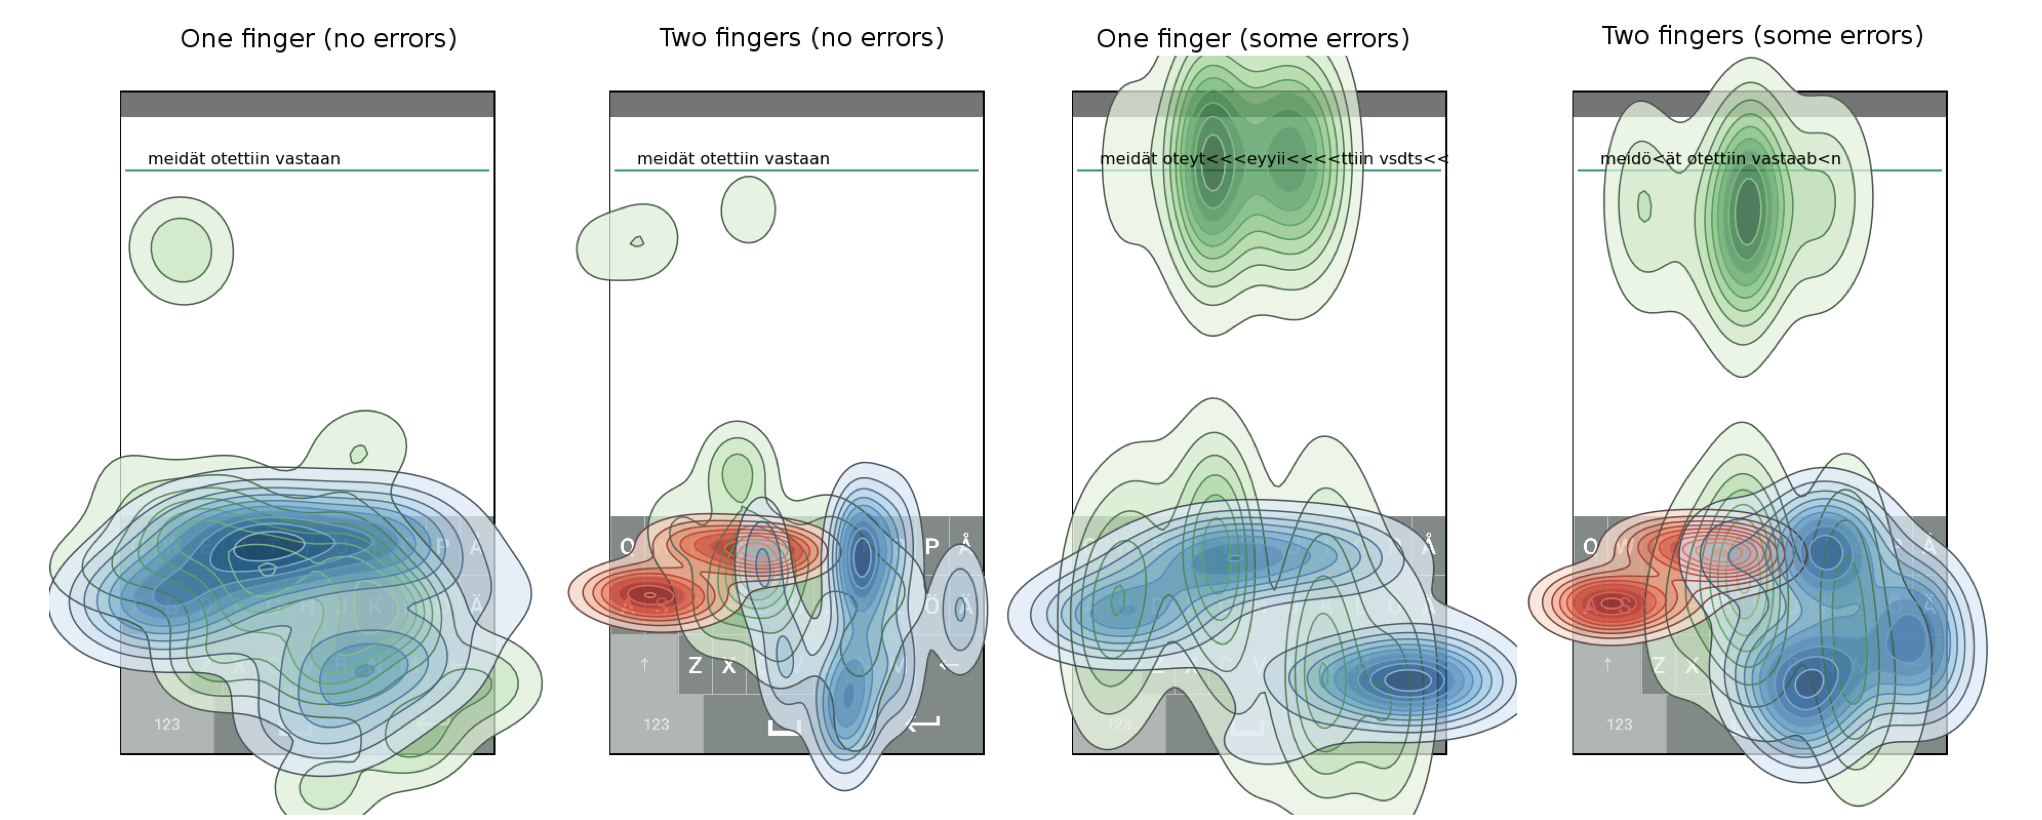
\includegraphics[width=12cm]{figures/fingermodel.png}
    \caption{A sample of finger typing model built from various users done by the work of \cite{jiangwe}. This allows us to understand user behaviours and various typing mechanisms which aids in designing interfaces better.
 }\label{fig:fingermodel}
\end{figure}

%\item The study of \cite{lee2018moving}
\item The work of \cite{kim2018impact} investigated on how impact activation can improve button pressing when testing in various fast-tapping experiments. Findings mention that impact activation significantly improves performance by the users. In music teaching systems, pressing the piano resembles an action of pressing a button and as such, the model built in this work can be used to understand and help the user improve in its piano key-pressing accuracies. 
\item The study of \cite{lee2019geometrically} constructed a predictive model that explains the effect of end-to-end latency on user error rates in a moving target. This was tested on moving-target selection games which have the same rhythm and synchronization effect as music teaching systems. In the paper they were able to address the latency that can offset from unintended effects. This model can be added in an augmented reality teaching system so that we can isolate expert and novice errors in understanding their actions and reactions in the immersive space. 
\item The study of \cite{liao2020button} performed analysis and simulations of buttons in FDVV models. Their focus was on modelling an FDVV model of a button and model the user's actions on pressing, force, displacement, vibration and velocity into a fitness metric that involves Bayesian Information Criteria. Their contribution highlights reducing the number of parameters, considering complexity penalty and how the simulations can compensate for these rendering. 
\end{itemize}
\section{Research Plan and Methodology}
The area of modeling, analyzing and investigating spatiotemporal pointing is relatively-new and much has been left unexplored. There are several attempts to understand and model basic human activities, their reaction and their cognitive loads while doing and being immersed in these spatiotemporal activities.\\

There are numerous papers and works on Augmented Reality Music Teaching Systems and most of their contributions are either on introducing a new ubiquituous interface, having practice and expert modes, improving the graphical rendering of the augmented visualizations. With the consideration of modeling and understanding spatiotemporal pointing within these augmented reality music teaching systems, there seems to be a lot of room to explore.\\

The proponent began with the prior research question of \textit{How might we model and understand the skills of a music expert and develop an interface that beginners can use to ease their music learning experiences}? We believe that to be able to build and understand these models, we can discover the different affordances and guidelines that we can use to design an interface that will help address this research question in mind. An overview of the research plan and methodology is described in Fig.\ref{fig:branches}. The green branches represent the theoretical background that needs to be verified using laboratory experiments. This allows the proponent to validate the research questions within the study.  The orange branches include an interdisciplinary investigation on spatiotemporal pointing and sensorimotor parameters that allow the research to validate its hypothesis involving cognitive load. The middle element in highlight capitalizes on the results of both orange and green branches, \textbf{Understanding Novice and Expert Users in AR Piano Teaching Systems with Spatiotemporal Pointing}, is the intended focus of the dissertation. 

\begin{landscape}
\begin{figure}[h]
\centering
 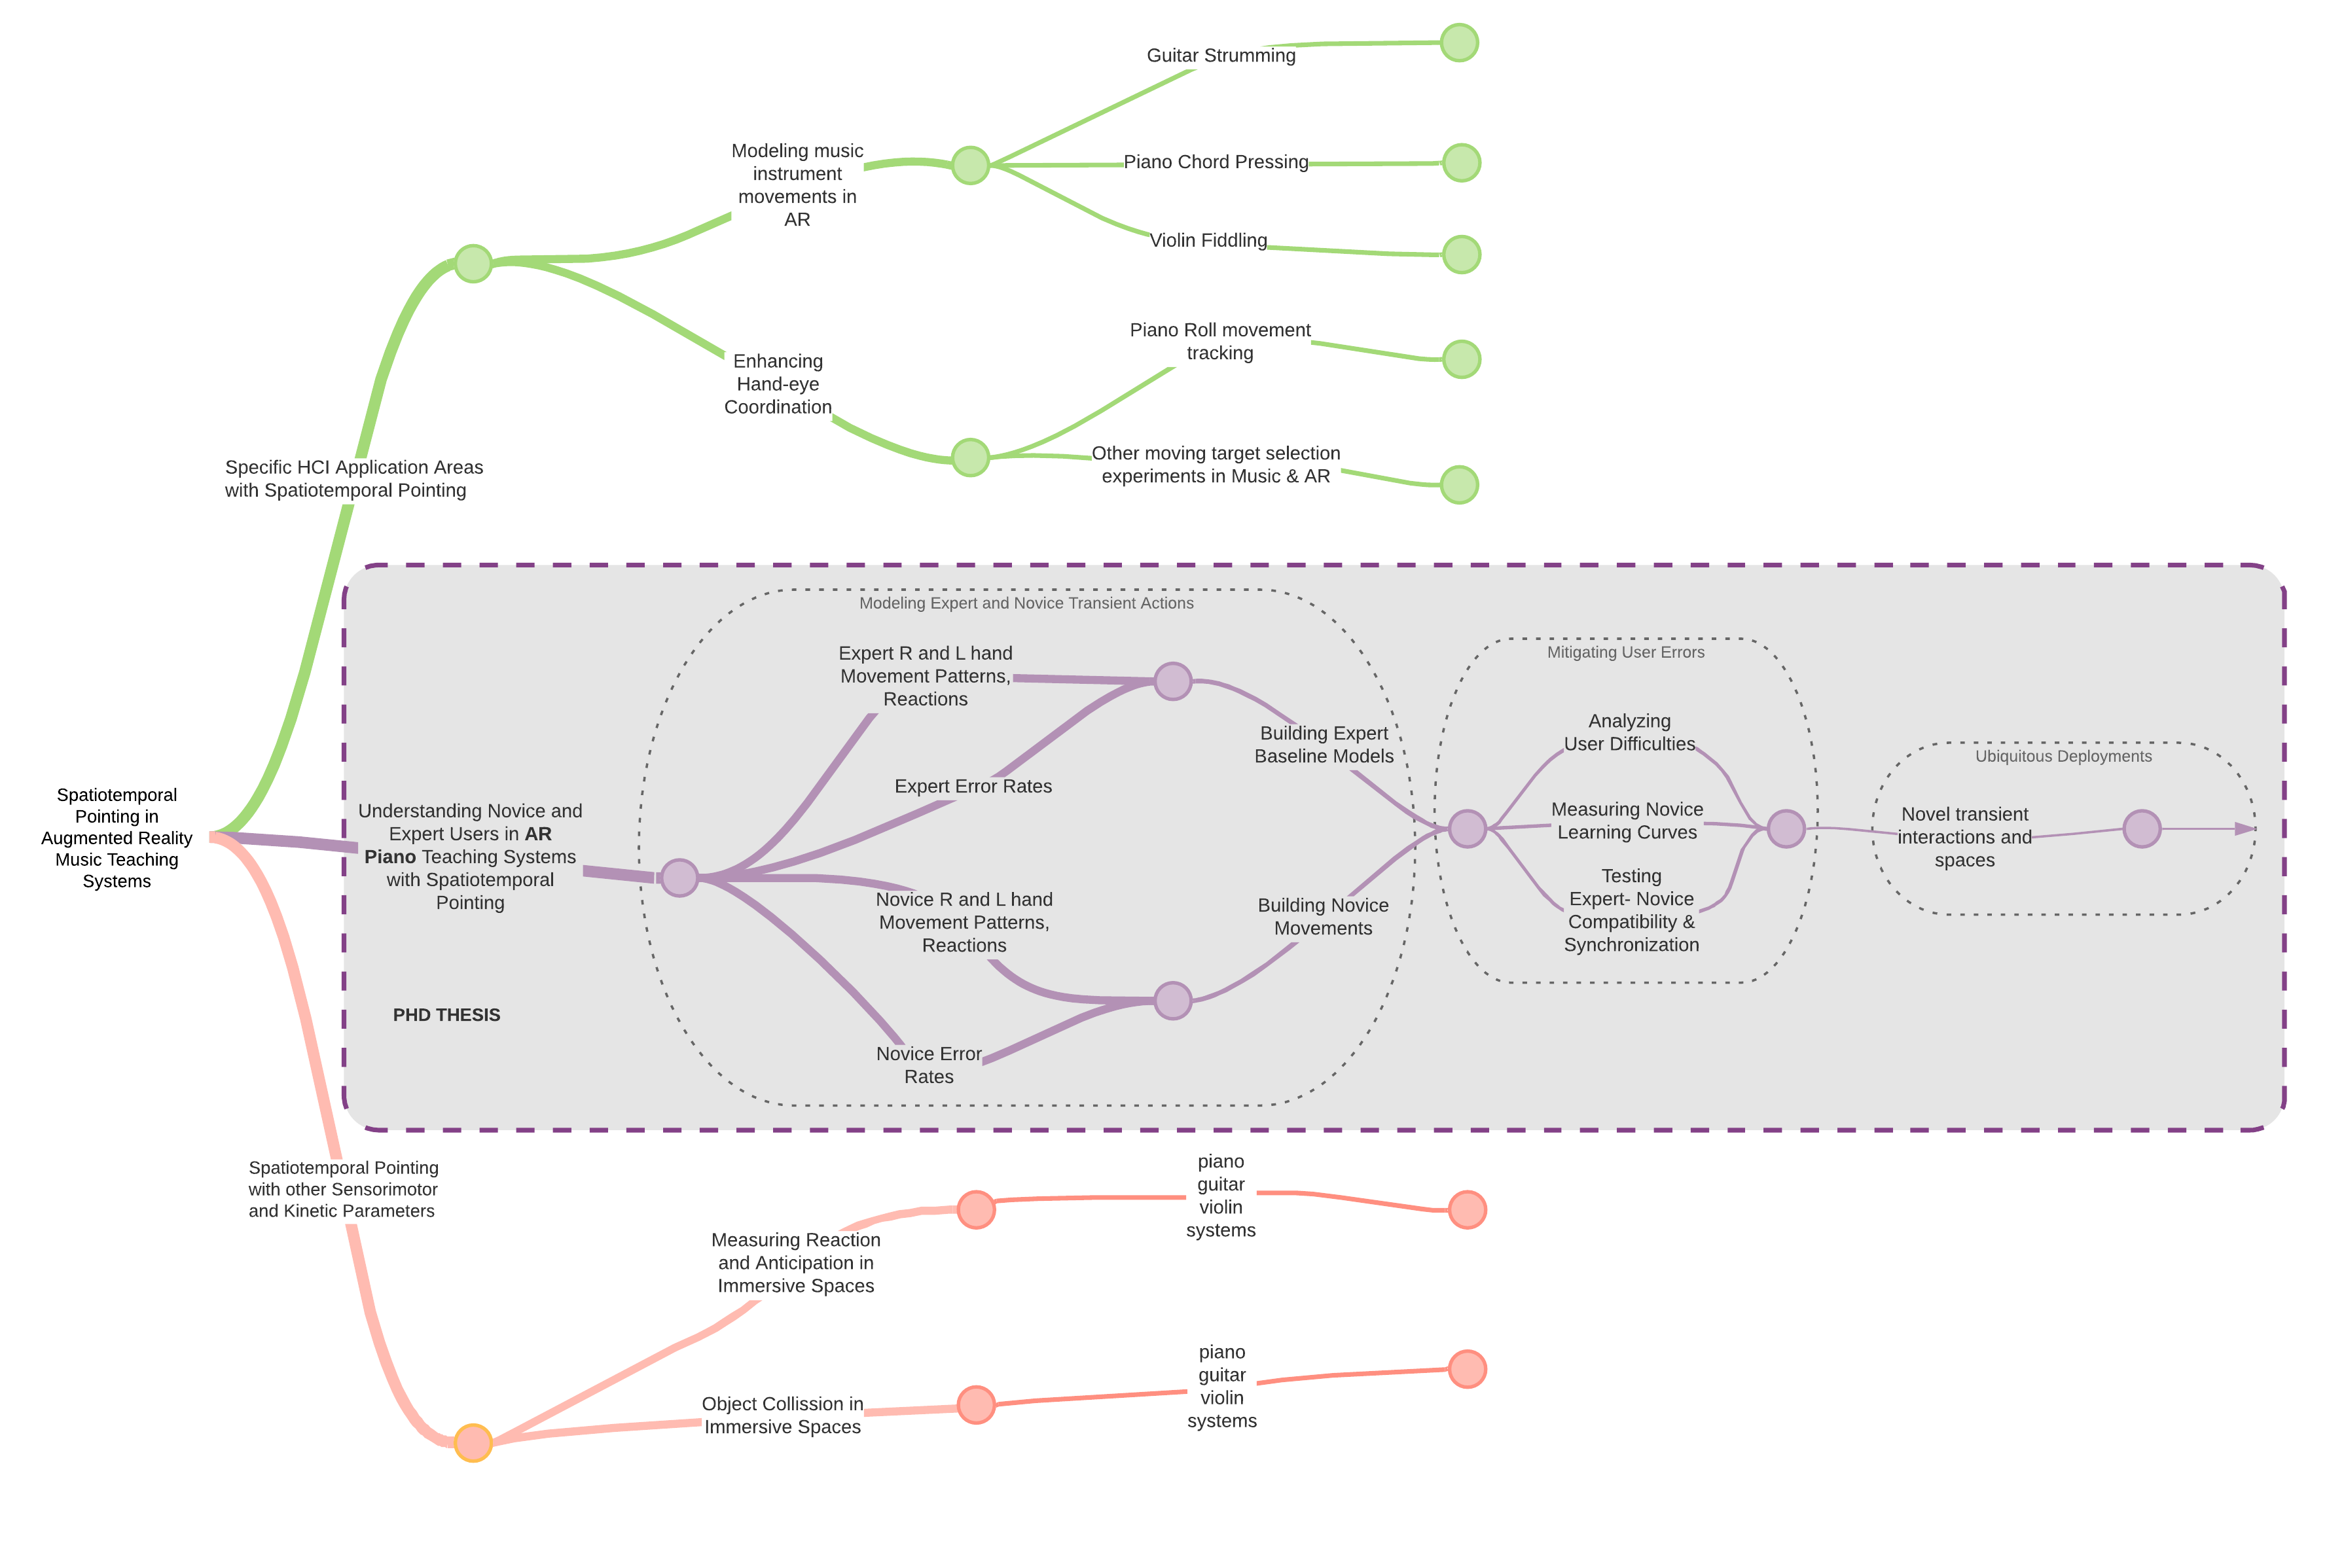
\includegraphics[width=\columnwidth\textheight]{figures/branches.png}
    \caption{An overview of the research branches showing breadth and depth. Each branch represents an experiment which will be part of the methodology in this proposal. Each node in the diagram is targetted  as a concrete contribution leading to a publication.
 }\label{fig:branches}
\end{figure}
\end{landscape}

\subsection{Research Questions}
The research proposal shall focus on how we can model the actions, reactions and cognitive load of users of various augmented reality music teaching systems. It shall cover breadth of use-cases, and tasks that consider user activities while being immersed in these environments. Such tasks include strumming (guitar), fiddling (violin), and pressing (piano) in immersive spaces. We can dive specifically into augmented reality piano teaching systems  and use the initial models from these broad music instruments as standards and baselines. To understand how the research can be executed, we raise the following questions: 
\begin{enumerate}
    \item How do experts and novices interact with a musical instrument?\\
    Hypothesis: Experts and novices interact differently with a music instrument be it a physical or an virtual one. 
    \item How can we model the actions, reactions, thought processes of both expert and novice users when using an augmented reality music system?\\
    Hypothesis: Expert models can be established as an ideal baseline or target performance for novice users. 
    \item What features in an augmented reality music teaching system can we introduce to design an interface for novice users?\\
    Hypothesis: Understanding novice user models and expert user models can allow us to discover gaps in skills that can be prioritized in the design of these immersive interfaces. 
    \item How do we re-imagine novice interactions with augmented reality music teaching systems built from their user models?\\
    Hypothesis: By designing an immersive interface built with expert user models as baselines, we can understand better the cognitive load experienced novices which affects learning. 
    \item What is the relationship between spatiotemporal pointing difficulty and musical skills difficulty?\\
    Hypothesis: Reducing difficulty in spatiotemporal pointing can reduce cognitive load that can help novices in mastering their music skills. 
\end{enumerate}
\subsection{Methodology}
This research shall have five (5) distinct intermediary phases that are reflected and seen on Fig \ref{fig:branches}. These are:
\begin{itemize}
    \item (Pre-A) Pre-Dissertation Phase A: Validating Specific Music HCI Application Areas with Spatiotemporal Pointing
    \item (Pre-B) Pre-Dissertation Phase B: Bridging Spatiotemporal Pointing with other Sensorimotor and Kinetic Parameters in Music Teaching Systems
    \item (Diss A) Dissertation Phase A: Building Models of Expert and Novice Transient Actions
    \item (Diss B) Dissertation Phase B: Mitigating User Errors in Spatiotemporal Pointing
    \item (Diss C) Dissertation Phase C: Deploying Ubiquitous Augmented Reality Music Teaching Systems\\
\end{itemize}

Phase Pre-A are laboratory experiments where musicians of various levels and instruments will be recruited to play the guitar, violin and piano. In these experiments we shall deploy sensors that capture their movement. We refer to these as traditional data collection setups. This phase has a counterpart setup which we shall refer to as Mixed Reality setups. Here, the same musicians shall be immersed in a virtual environment and their usage data shall be collected while interacting with real-world tangible artifacts (guitar, piano, violin). This phase shall allow us to capture enough data that can be used to build usage models. These models can allow us to understand and compare spatiotemporal movement with music instruments vs movements in traditional music setups. These will then be used as baselines for the succeeding phases of this research. \\

Phase Pre-B are laboratory experiments where we shall incorporate other sensors and techniques that can be used to collect, measure and understand cognitive load. While Phase Pre-A shall focus on the movements like strumming, fiddling and key-pressing, Phase Pre-B shall include methods that acquire and measure signals related to affect such as: Galvanic Sensor Responsor (GSR), Electroencephalogy (ECG) and other inputs. These multimodal signals will be captured during experiments involving music instruments with the aim of measuring and understanding temporal activities such as hand-eye coordination in fiddling, pressing and strumming. This phase shall also cover related topics to spatiotemporal pointing that may affect cognitive load in immersive spaces such as object collision, piano roll visualizations and rhythm-based synchronization activities. This phase is important in helping us understand if there are possible relationships between cognitive load, and the factors that affect spatiotemporal pointing. This way, we can gauge and identify factors in immersive and augmented visualizations that may affect learning ultimately. \\

Phase Diss A shall benefit from the results of intermediary phases Pre-A and Pre-B. Phases Diss A to C will be done in succession and relative pre-requisites. These phases have been designed with the hypotheses in mind. Phase Diss A shall be the formative phase of this dissertation. It shall cover several experiments involving Novice and Expert Piano users. The phase drills down on investigating whether there are differences in both left and hand users between expert and novice piano users. Their movement patterns, hand-eye coordination, and more importantly their error rates will be observed, collected and modelled. Models of expert movement patterns, error rates, reaction times will be built and used as baseline models in order to compare and analyze Novice models. This phase shall allow us to understand if there are observable differences in between how novices and experts use the piano. The findings in this phase shall establish groundwork in identifying guidelines, patterns, design affordances and even rules that can be used to help novices transition into becoming more experienced users similar or close to their expert counterparts. \\

Phase Diss B shall be a series of exploratory experiments that attempt to reconcile the assumed differences between expert and novice users. The ultimate goal of this phase is to understand these differences, the learning curves, user pain points towards the design and development of an immersive and/or ubiquitous piano teaching space. This phase will include compatibility tests, expert-novice synchronization studies, and person-specific user studies that contribute to understanding the human factors involved in spatiotemporal activities in immersive piano systems. The goal of this phase is to come up with an initial design for an immersive space that feature novel transient interactions that aid in learning piano. \\

Phase Diss C shall be the summative phase of this research. While everything designed in this phase are based on the assumptions and successess of the previous phases, it is important to note that this phase shall cement the intended contribution of the proponent. Deploying systems and testing usability of these spaces will be the core activity in this phase. These test phases will be iterative. Findings from iterative tests shall provide affordances for a better design of the interface which shall be used for the succeeding iterative tests. 
\section{Contribution}
The works of \cite{liao2020button, lee2019geometrically} have established the foundation on modeling and measuring basic actions in immersive spaces. Their work  at the same time has addressed minimizing latency in these spaces and button setups. This research will focus on understanding user models in augmented reality music teaching spaces and how to build and analyze them. It will contribute to better understanding of the differences between expert and novice musicians and how cognitive load affects their learning within these immersive spaces. The findings of the proposed research will be very useful to the research community interested in Augmented Reality, Music Teaching Systems, interface design. 
\bibliographystyle{apacite}
\bibliography{references}

\end{document}
